\documentclass[twoside]{book}

% Packages required by doxygen
\usepackage{fixltx2e}
\usepackage{calc}
\usepackage{doxygen}
\usepackage[export]{adjustbox} % also loads graphicx
\usepackage{graphicx}
\usepackage[utf8]{inputenc}
\usepackage{makeidx}
\usepackage{multicol}
\usepackage{multirow}
\PassOptionsToPackage{warn}{textcomp}
\usepackage{textcomp}
\usepackage[nointegrals]{wasysym}
\usepackage[table]{xcolor}

% Font selection
\usepackage[T1]{fontenc}
\usepackage[scaled=.90]{helvet}
\usepackage{courier}
\usepackage{amssymb}
\usepackage{sectsty}
\renewcommand{\familydefault}{\sfdefault}
\allsectionsfont{%
  \fontseries{bc}\selectfont%
  \color{darkgray}%
}
\renewcommand{\DoxyLabelFont}{%
  \fontseries{bc}\selectfont%
  \color{darkgray}%
}
\newcommand{\+}{\discretionary{\mbox{\scriptsize$\hookleftarrow$}}{}{}}

% Page & text layout
\usepackage{geometry}
\geometry{%
  a4paper,%
  top=2.5cm,%
  bottom=2.5cm,%
  left=2.5cm,%
  right=2.5cm%
}
\tolerance=750
\hfuzz=15pt
\hbadness=750
\setlength{\emergencystretch}{15pt}
\setlength{\parindent}{0cm}
\setlength{\parskip}{3ex plus 2ex minus 2ex}
\makeatletter
\renewcommand{\paragraph}{%
  \@startsection{paragraph}{4}{0ex}{-1.0ex}{1.0ex}{%
    \normalfont\normalsize\bfseries\SS@parafont%
  }%
}
\renewcommand{\subparagraph}{%
  \@startsection{subparagraph}{5}{0ex}{-1.0ex}{1.0ex}{%
    \normalfont\normalsize\bfseries\SS@subparafont%
  }%
}
\makeatother

% Headers & footers
\usepackage{fancyhdr}
\pagestyle{fancyplain}
\fancyhead[LE]{\fancyplain{}{\bfseries\thepage}}
\fancyhead[CE]{\fancyplain{}{}}
\fancyhead[RE]{\fancyplain{}{\bfseries\leftmark}}
\fancyhead[LO]{\fancyplain{}{\bfseries\rightmark}}
\fancyhead[CO]{\fancyplain{}{}}
\fancyhead[RO]{\fancyplain{}{\bfseries\thepage}}
\fancyfoot[LE]{\fancyplain{}{}}
\fancyfoot[CE]{\fancyplain{}{}}
\fancyfoot[RE]{\fancyplain{}{\bfseries\scriptsize Generated by Doxygen }}
\fancyfoot[LO]{\fancyplain{}{\bfseries\scriptsize Generated by Doxygen }}
\fancyfoot[CO]{\fancyplain{}{}}
\fancyfoot[RO]{\fancyplain{}{}}
\renewcommand{\footrulewidth}{0.4pt}
\renewcommand{\chaptermark}[1]{%
  \markboth{#1}{}%
}
\renewcommand{\sectionmark}[1]{%
  \markright{\thesection\ #1}%
}

% Indices & bibliography
\usepackage{natbib}
\usepackage[titles]{tocloft}
\setcounter{tocdepth}{3}
\setcounter{secnumdepth}{5}
\makeindex

% Hyperlinks (required, but should be loaded last)
\usepackage{ifpdf}
\ifpdf
  \usepackage[pdftex,pagebackref=true]{hyperref}
\else
  \usepackage[ps2pdf,pagebackref=true]{hyperref}
\fi
\hypersetup{%
  colorlinks=true,%
  linkcolor=blue,%
  citecolor=blue,%
  unicode%
}

% Custom commands
\newcommand{\clearemptydoublepage}{%
  \newpage{\pagestyle{empty}\cleardoublepage}%
}

\usepackage{caption}
\captionsetup{labelsep=space,justification=centering,font={bf},singlelinecheck=off,skip=4pt,position=top}

%===== C O N T E N T S =====

\begin{document}

% Titlepage & ToC
\hypersetup{pageanchor=false,
             bookmarksnumbered=true,
             pdfencoding=unicode
            }
\pagenumbering{alph}
\begin{titlepage}
\vspace*{7cm}
\begin{center}%
{\Large Stephen Cyr, A00991588, Lab 5 }\\
\vspace*{1cm}
{\large Generated by Doxygen 1.8.12}\\
\end{center}
\end{titlepage}
\clearemptydoublepage
\pagenumbering{roman}
\tableofcontents
\clearemptydoublepage
\pagenumbering{arabic}
\hypersetup{pageanchor=true}

%--- Begin generated contents ---
\chapter{Hierarchical Index}
\section{Class Hierarchy}
This inheritance list is sorted roughly, but not completely, alphabetically\+:\begin{DoxyCompactList}
\item \contentsline{section}{C\+Base4618}{\pageref{class_c_base4618}}{}
\begin{DoxyCompactList}
\item \contentsline{section}{C\+Pong}{\pageref{class_c_pong}}{}
\end{DoxyCompactList}
\item \contentsline{section}{C\+Control}{\pageref{class_c_control}}{}
\end{DoxyCompactList}

\chapter{Class Index}
\section{Class List}
Here are the classes, structs, unions and interfaces with brief descriptions\+:\begin{DoxyCompactList}
\item\contentsline{section}{\hyperlink{class_c_base4618}{C\+Base4618} \\*Initializes Mat and \hyperlink{class_c_control}{C\+Control} objects }{\pageref{class_c_base4618}}{}
\item\contentsline{section}{\hyperlink{class_c_control}{C\+Control} \\*Communicates through serail port }{\pageref{class_c_control}}{}
\item\contentsline{section}{\hyperlink{class_c_pong}{C\+Pong} \\*Runs the game pong }{\pageref{class_c_pong}}{}
\end{DoxyCompactList}

\chapter{Class Documentation}
\hypertarget{class_c_base4618}{}\section{C\+Base4618 Class Reference}
\label{class_c_base4618}\index{C\+Base4618@{C\+Base4618}}


initializes Mat and \hyperlink{class_c_control}{C\+Control} objects  




{\ttfamily \#include $<$C\+Base4618.\+h$>$}

Inheritance diagram for C\+Base4618\+:\begin{figure}[H]
\begin{center}
\leavevmode
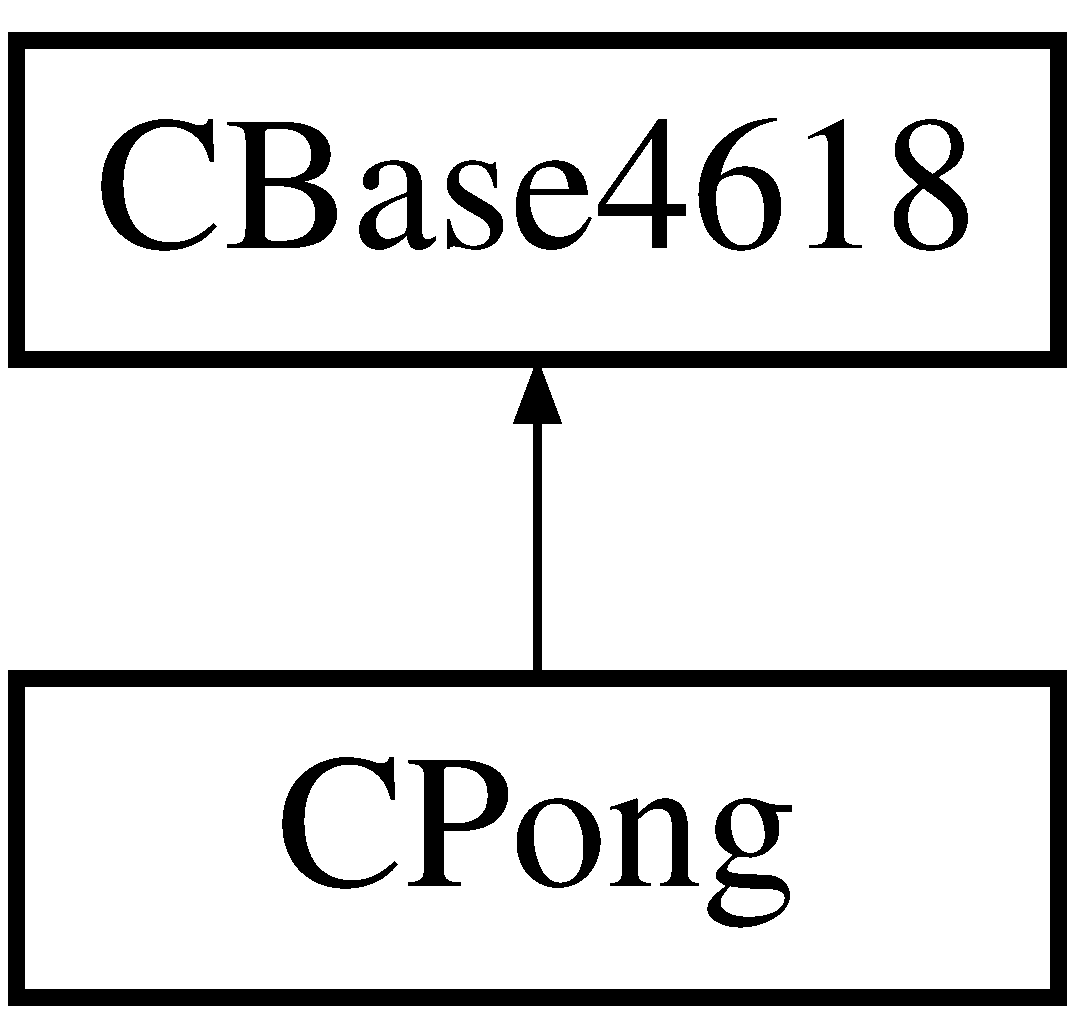
\includegraphics[height=2.000000cm]{class_c_base4618}
\end{center}
\end{figure}
\subsection*{Public Member Functions}
\begin{DoxyCompactItemize}
\item 
\hyperlink{class_c_base4618_abe2aad021452c08dd4a5726b44c5a0b7}{C\+Base4618} ()
\begin{DoxyCompactList}\small\item\em Contructor creates. \end{DoxyCompactList}\item 
\hyperlink{class_c_base4618_a22c0de299cef06c4ef49ace3a5b0be52}{$\sim$\+C\+Base4618} ()
\begin{DoxyCompactList}\small\item\em \hyperlink{class_c_base4618}{C\+Base4618} deconstructor. \end{DoxyCompactList}\item 
void \hyperlink{class_c_base4618_a535e816d735d10d6048dd39cd893d393}{run} ()
\begin{DoxyCompactList}\small\item\em calls udpdate and draw on a loop until until it receivs q key \end{DoxyCompactList}\end{DoxyCompactItemize}
\subsection*{Protected Member Functions}
\begin{DoxyCompactItemize}
\item 
virtual void \hyperlink{class_c_base4618_a1e2f3c16eb99b5bfdd5d5254aee39ee6}{update} ()=0
\begin{DoxyCompactList}\small\item\em virtual method update reads data from com port and updates the x and y positions \end{DoxyCompactList}\item 
virtual void \hyperlink{class_c_base4618_a0987bf28e9beed4753d3628fcddc3315}{draw} ()=0
\begin{DoxyCompactList}\small\item\em virtual method draws a line in a direction on \+\_\+canvas depending on x and y values from update \end{DoxyCompactList}\end{DoxyCompactItemize}
\subsection*{Protected Attributes}
\begin{DoxyCompactItemize}
\item 
\hypertarget{class_c_base4618_a1b925f757247b33ca2072f777f24582d}{}\label{class_c_base4618_a1b925f757247b33ca2072f777f24582d} 
cv\+::\+Mat \hyperlink{class_c_base4618_a1b925f757247b33ca2072f777f24582d}{\+\_\+canvas}
\begin{DoxyCompactList}\small\item\em Mat object to create drawing window. \end{DoxyCompactList}\item 
\hypertarget{class_c_base4618_ac838c5eaf9edfb1e607bd90e4e246a37}{}\label{class_c_base4618_ac838c5eaf9edfb1e607bd90e4e246a37} 
\hyperlink{class_c_control}{C\+Control} \hyperlink{class_c_base4618_ac838c5eaf9edfb1e607bd90e4e246a37}{sketch\+\_\+contr}
\begin{DoxyCompactList}\small\item\em \hyperlink{class_c_control}{C\+Control} opject to get data from com port. \end{DoxyCompactList}\end{DoxyCompactItemize}


\subsection{Detailed Description}
initializes Mat and \hyperlink{class_c_control}{C\+Control} objects 

Initializes Mat and \hyperlink{class_c_control}{C\+Control} objects and creates function decriptors for update and draw, and then run runs them on a loop

\begin{DoxyAuthor}{Author}
Stephen Cyr 
\end{DoxyAuthor}


\subsection{Constructor \& Destructor Documentation}
\hypertarget{class_c_base4618_abe2aad021452c08dd4a5726b44c5a0b7}{}\label{class_c_base4618_abe2aad021452c08dd4a5726b44c5a0b7} 
\index{C\+Base4618@{C\+Base4618}!C\+Base4618@{C\+Base4618}}
\index{C\+Base4618@{C\+Base4618}!C\+Base4618@{C\+Base4618}}
\subsubsection{\texorpdfstring{C\+Base4618()}{CBase4618()}}
{\footnotesize\ttfamily C\+Base4618\+::\+C\+Base4618 (\begin{DoxyParamCaption}{ }\end{DoxyParamCaption})}



Contructor creates. 


\begin{DoxyParams}{Parameters}
{\em none} & \\
\hline
\end{DoxyParams}
\begin{DoxyReturn}{Returns}
nothing 
\end{DoxyReturn}
\hypertarget{class_c_base4618_a22c0de299cef06c4ef49ace3a5b0be52}{}\label{class_c_base4618_a22c0de299cef06c4ef49ace3a5b0be52} 
\index{C\+Base4618@{C\+Base4618}!````~C\+Base4618@{$\sim$\+C\+Base4618}}
\index{````~C\+Base4618@{$\sim$\+C\+Base4618}!C\+Base4618@{C\+Base4618}}
\subsubsection{\texorpdfstring{$\sim$\+C\+Base4618()}{~CBase4618()}}
{\footnotesize\ttfamily C\+Base4618\+::$\sim$\+C\+Base4618 (\begin{DoxyParamCaption}{ }\end{DoxyParamCaption})}



\hyperlink{class_c_base4618}{C\+Base4618} deconstructor. 


\begin{DoxyParams}{Parameters}
{\em none} & \\
\hline
\end{DoxyParams}
\begin{DoxyReturn}{Returns}
nothing 
\end{DoxyReturn}


\subsection{Member Function Documentation}
\hypertarget{class_c_base4618_a0987bf28e9beed4753d3628fcddc3315}{}\label{class_c_base4618_a0987bf28e9beed4753d3628fcddc3315} 
\index{C\+Base4618@{C\+Base4618}!draw@{draw}}
\index{draw@{draw}!C\+Base4618@{C\+Base4618}}
\subsubsection{\texorpdfstring{draw()}{draw()}}
{\footnotesize\ttfamily virtual void C\+Base4618\+::draw (\begin{DoxyParamCaption}{ }\end{DoxyParamCaption})\hspace{0.3cm}{\ttfamily [protected]}, {\ttfamily [pure virtual]}}



virtual method draws a line in a direction on \+\_\+canvas depending on x and y values from update 


\begin{DoxyParams}{Parameters}
{\em none} & \\
\hline
\end{DoxyParams}
\begin{DoxyReturn}{Returns}
nothing 
\end{DoxyReturn}


Implemented in \hyperlink{class_c_pong_ae5c14ff09d074474ffd4f220b21dc00f}{C\+Pong}.

\hypertarget{class_c_base4618_a535e816d735d10d6048dd39cd893d393}{}\label{class_c_base4618_a535e816d735d10d6048dd39cd893d393} 
\index{C\+Base4618@{C\+Base4618}!run@{run}}
\index{run@{run}!C\+Base4618@{C\+Base4618}}
\subsubsection{\texorpdfstring{run()}{run()}}
{\footnotesize\ttfamily void C\+Base4618\+::run (\begin{DoxyParamCaption}{ }\end{DoxyParamCaption})}



calls udpdate and draw on a loop until until it receivs q key 


\begin{DoxyParams}{Parameters}
{\em none} & \\
\hline
\end{DoxyParams}
\begin{DoxyReturn}{Returns}
nothing 
\end{DoxyReturn}
\hypertarget{class_c_base4618_a1e2f3c16eb99b5bfdd5d5254aee39ee6}{}\label{class_c_base4618_a1e2f3c16eb99b5bfdd5d5254aee39ee6} 
\index{C\+Base4618@{C\+Base4618}!update@{update}}
\index{update@{update}!C\+Base4618@{C\+Base4618}}
\subsubsection{\texorpdfstring{update()}{update()}}
{\footnotesize\ttfamily virtual void C\+Base4618\+::update (\begin{DoxyParamCaption}{ }\end{DoxyParamCaption})\hspace{0.3cm}{\ttfamily [protected]}, {\ttfamily [pure virtual]}}



virtual method update reads data from com port and updates the x and y positions 


\begin{DoxyParams}{Parameters}
{\em none} & \\
\hline
\end{DoxyParams}
\begin{DoxyReturn}{Returns}
nothing 
\end{DoxyReturn}


Implemented in \hyperlink{class_c_pong_abdf0d44329b40d14863ba134b031435a}{C\+Pong}.



The documentation for this class was generated from the following files\+:\begin{DoxyCompactItemize}
\item 
C\+Base4618.\+h\item 
C\+Base4618.\+cpp\end{DoxyCompactItemize}

\hypertarget{class_c_control}{}\section{C\+Control Class Reference}
\label{class_c_control}\index{C\+Control@{C\+Control}}


Communicates through serail port.  




{\ttfamily \#include $<$C\+Control.\+h$>$}

\subsection*{Public Member Functions}
\begin{DoxyCompactItemize}
\item 
\hyperlink{class_c_control_a6498500ff403327b5770a3acebed1d93}{C\+Control} ()
\begin{DoxyCompactList}\small\item\em \hyperlink{class_c_control}{C\+Control} constructor. \end{DoxyCompactList}\item 
\hyperlink{class_c_control_ab2ae420ef75b010c0c9078e597781105}{$\sim$\+C\+Control} ()
\begin{DoxyCompactList}\small\item\em \hyperlink{class_c_control}{C\+Control} destructor. \end{DoxyCompactList}\item 
void \hyperlink{class_c_control_a3d1384d0e1ee2a4a478a798b46457468}{init\+\_\+com} (int comport)
\begin{DoxyCompactList}\small\item\em initalizes serial communication with specified com port \end{DoxyCompactList}\item 
bool \hyperlink{class_c_control_a0bad8e51e54cb6f1e2a7b51d3a3940d3}{get\+\_\+data} (int type, int channel, int \&result)
\begin{DoxyCompactList}\small\item\em sends a request for a type of data at a pin, and reads return data at com port \end{DoxyCompactList}\item 
bool \hyperlink{class_c_control_a13f557815616ef66a8f5dd4b725d8c32}{set\+\_\+data} (int type, int channel, int val)
\begin{DoxyCompactList}\small\item\em sends a signal to be outputed on a specified channel \end{DoxyCompactList}\item 
bool \hyperlink{class_c_control_a0b4ca36ae9a4b2a1ab98992ab35f2209}{get\+\_\+analog} (int, int, int \&, int \&)
\begin{DoxyCompactList}\small\item\em Calls get\+\_\+data function and returns data type and analog data and percent. \end{DoxyCompactList}\item 
bool \hyperlink{class_c_control_ad4a408390baa24847dc16cb49b64ddad}{get\+\_\+butt} (int \&, int, int=0)
\begin{DoxyCompactList}\small\item\em Calls get\+\_\+data function to specificly get a digital signal. \end{DoxyCompactList}\end{DoxyCompactItemize}
\subsection*{Private Attributes}
\begin{DoxyCompactItemize}
\item 
\hypertarget{class_c_control_aef87fbcfdcd323b1fdcf41be993e006c}{}\label{class_c_control_aef87fbcfdcd323b1fdcf41be993e006c} 
Serial \hyperlink{class_c_control_aef87fbcfdcd323b1fdcf41be993e006c}{\+\_\+com}
\begin{DoxyCompactList}\small\item\em Serial object used for serial communication with com port. \end{DoxyCompactList}\item 
\hypertarget{class_c_control_acf72e99f9fd9b389300b435c145a3bcb}{}\label{class_c_control_acf72e99f9fd9b389300b435c145a3bcb} 
double \hyperlink{class_c_control_acf72e99f9fd9b389300b435c145a3bcb}{last\+\_\+push} = cv\+::get\+Tick\+Count()
\begin{DoxyCompactList}\small\item\em Time of last button push. \end{DoxyCompactList}\end{DoxyCompactItemize}


\subsection{Detailed Description}
Communicates through serail port. 

Initializes serial communication and has methods to read and write data to com port

\begin{DoxyAuthor}{Author}
Stephen Cyr 
\end{DoxyAuthor}


\subsection{Constructor \& Destructor Documentation}
\hypertarget{class_c_control_a6498500ff403327b5770a3acebed1d93}{}\label{class_c_control_a6498500ff403327b5770a3acebed1d93} 
\index{C\+Control@{C\+Control}!C\+Control@{C\+Control}}
\index{C\+Control@{C\+Control}!C\+Control@{C\+Control}}
\subsubsection{\texorpdfstring{C\+Control()}{CControl()}}
{\footnotesize\ttfamily C\+Control\+::\+C\+Control (\begin{DoxyParamCaption}{ }\end{DoxyParamCaption})}



\hyperlink{class_c_control}{C\+Control} constructor. 


\begin{DoxyParams}{Parameters}
{\em none} & \\
\hline
\end{DoxyParams}
\begin{DoxyReturn}{Returns}
nothing 
\end{DoxyReturn}
\hypertarget{class_c_control_ab2ae420ef75b010c0c9078e597781105}{}\label{class_c_control_ab2ae420ef75b010c0c9078e597781105} 
\index{C\+Control@{C\+Control}!````~C\+Control@{$\sim$\+C\+Control}}
\index{````~C\+Control@{$\sim$\+C\+Control}!C\+Control@{C\+Control}}
\subsubsection{\texorpdfstring{$\sim$\+C\+Control()}{~CControl()}}
{\footnotesize\ttfamily C\+Control\+::$\sim$\+C\+Control (\begin{DoxyParamCaption}{ }\end{DoxyParamCaption})}



\hyperlink{class_c_control}{C\+Control} destructor. 


\begin{DoxyParams}{Parameters}
{\em none} & \\
\hline
\end{DoxyParams}
\begin{DoxyReturn}{Returns}
nothing 
\end{DoxyReturn}


\subsection{Member Function Documentation}
\hypertarget{class_c_control_a0b4ca36ae9a4b2a1ab98992ab35f2209}{}\label{class_c_control_a0b4ca36ae9a4b2a1ab98992ab35f2209} 
\index{C\+Control@{C\+Control}!get\+\_\+analog@{get\+\_\+analog}}
\index{get\+\_\+analog@{get\+\_\+analog}!C\+Control@{C\+Control}}
\subsubsection{\texorpdfstring{get\+\_\+analog()}{get\_analog()}}
{\footnotesize\ttfamily bool C\+Control\+::get\+\_\+analog (\begin{DoxyParamCaption}\item[{int}]{type,  }\item[{int}]{channel,  }\item[{int \&}]{result,  }\item[{int \&}]{perc\+\_\+result }\end{DoxyParamCaption})}



Calls get\+\_\+data function and returns data type and analog data and percent. 


\begin{DoxyParams}{Parameters}
{\em int} & specifying data type, int specifying channel, memory address for data, and memory address for percent \\
\hline
\end{DoxyParams}
\begin{DoxyReturn}{Returns}
booling expresion 
\end{DoxyReturn}
\hypertarget{class_c_control_ad4a408390baa24847dc16cb49b64ddad}{}\label{class_c_control_ad4a408390baa24847dc16cb49b64ddad} 
\index{C\+Control@{C\+Control}!get\+\_\+butt@{get\+\_\+butt}}
\index{get\+\_\+butt@{get\+\_\+butt}!C\+Control@{C\+Control}}
\subsubsection{\texorpdfstring{get\+\_\+butt()}{get\_butt()}}
{\footnotesize\ttfamily bool C\+Control\+::get\+\_\+butt (\begin{DoxyParamCaption}\item[{int \&}]{result,  }\item[{int}]{butt,  }\item[{int}]{type = {\ttfamily 0} }\end{DoxyParamCaption})}



Calls get\+\_\+data function to specificly get a digital signal. 


\begin{DoxyParams}{Parameters}
{\em int} & specifying data type, int specifying channel, memory address for data, and memory address for percent \\
\hline
\end{DoxyParams}
\begin{DoxyReturn}{Returns}
booling expresion 
\end{DoxyReturn}
\hypertarget{class_c_control_a0bad8e51e54cb6f1e2a7b51d3a3940d3}{}\label{class_c_control_a0bad8e51e54cb6f1e2a7b51d3a3940d3} 
\index{C\+Control@{C\+Control}!get\+\_\+data@{get\+\_\+data}}
\index{get\+\_\+data@{get\+\_\+data}!C\+Control@{C\+Control}}
\subsubsection{\texorpdfstring{get\+\_\+data()}{get\_data()}}
{\footnotesize\ttfamily bool C\+Control\+::get\+\_\+data (\begin{DoxyParamCaption}\item[{int}]{type,  }\item[{int}]{channel,  }\item[{int \&}]{result }\end{DoxyParamCaption})}



sends a request for a type of data at a pin, and reads return data at com port 


\begin{DoxyParams}{Parameters}
{\em int} & specifying data type, int specifying what channel, and memory address of int to store response \\
\hline
\end{DoxyParams}
\begin{DoxyReturn}{Returns}
bool expression 
\end{DoxyReturn}
\hypertarget{class_c_control_a3d1384d0e1ee2a4a478a798b46457468}{}\label{class_c_control_a3d1384d0e1ee2a4a478a798b46457468} 
\index{C\+Control@{C\+Control}!init\+\_\+com@{init\+\_\+com}}
\index{init\+\_\+com@{init\+\_\+com}!C\+Control@{C\+Control}}
\subsubsection{\texorpdfstring{init\+\_\+com()}{init\_com()}}
{\footnotesize\ttfamily void C\+Control\+::init\+\_\+com (\begin{DoxyParamCaption}\item[{int}]{comport }\end{DoxyParamCaption})}



initalizes serial communication with specified com port 


\begin{DoxyParams}{Parameters}
{\em integer} & specifying com port \\
\hline
\end{DoxyParams}
\begin{DoxyReturn}{Returns}
nothing 
\end{DoxyReturn}
\hypertarget{class_c_control_a13f557815616ef66a8f5dd4b725d8c32}{}\label{class_c_control_a13f557815616ef66a8f5dd4b725d8c32} 
\index{C\+Control@{C\+Control}!set\+\_\+data@{set\+\_\+data}}
\index{set\+\_\+data@{set\+\_\+data}!C\+Control@{C\+Control}}
\subsubsection{\texorpdfstring{set\+\_\+data()}{set\_data()}}
{\footnotesize\ttfamily bool C\+Control\+::set\+\_\+data (\begin{DoxyParamCaption}\item[{int}]{type,  }\item[{int}]{channel,  }\item[{int}]{val }\end{DoxyParamCaption})}



sends a signal to be outputed on a specified channel 


\begin{DoxyParams}{Parameters}
{\em int} & specifying data type, int specifying channel, and int specifying value for pin \\
\hline
\end{DoxyParams}
\begin{DoxyReturn}{Returns}
booling expression 
\end{DoxyReturn}


The documentation for this class was generated from the following files\+:\begin{DoxyCompactItemize}
\item 
C\+Control.\+h\item 
C\+Control.\+cpp\end{DoxyCompactItemize}

\hypertarget{class_c_pong}{}\section{C\+Pong Class Reference}
\label{class_c_pong}\index{C\+Pong@{C\+Pong}}


Runs the game pong.  




{\ttfamily \#include $<$C\+Pong.\+h$>$}

Inheritance diagram for C\+Pong\+:\begin{figure}[H]
\begin{center}
\leavevmode
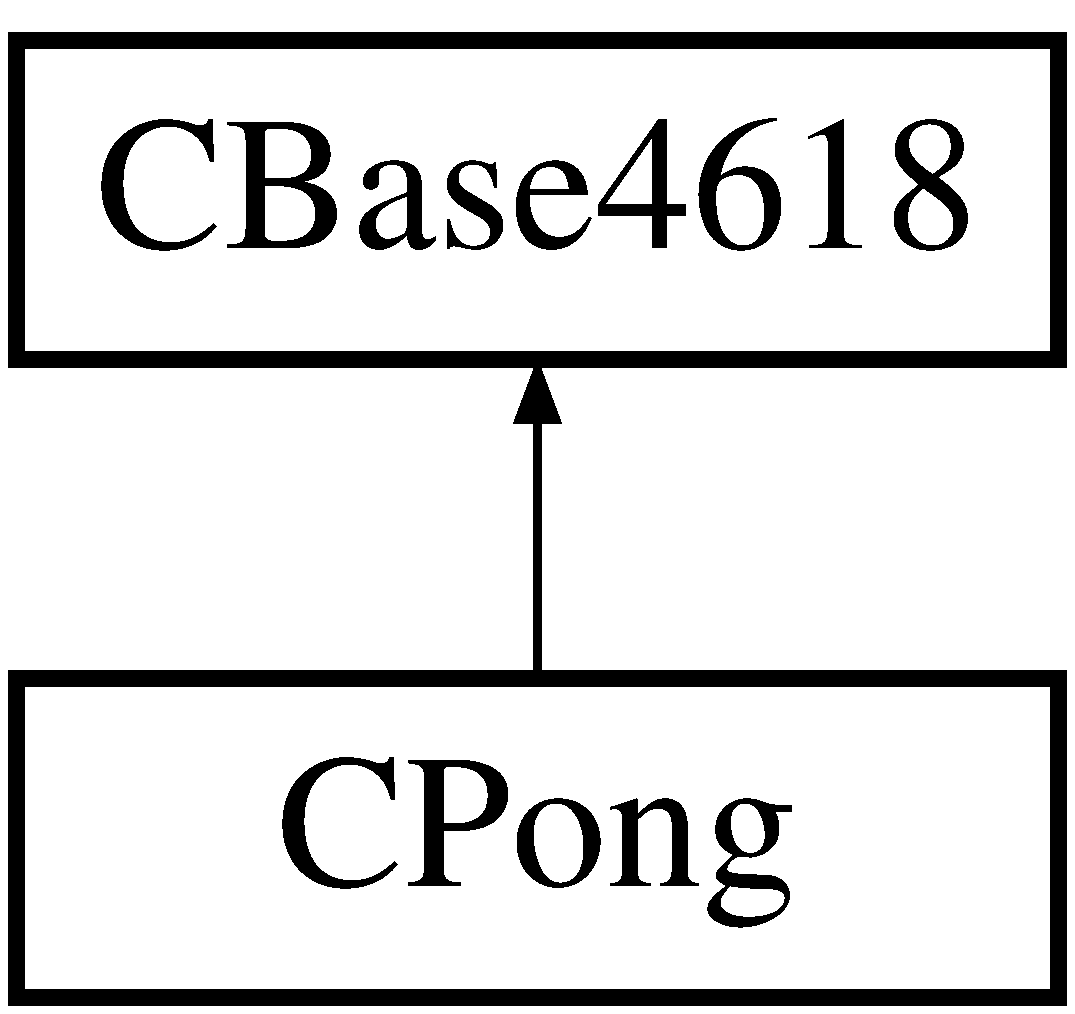
\includegraphics[height=2.000000cm]{class_c_pong}
\end{center}
\end{figure}
\subsection*{Public Member Functions}
\begin{DoxyCompactItemize}
\item 
\hyperlink{class_c_pong_ac118507edc4d9cc2dd1d2f1d9e88fa45}{C\+Pong} (Size dim=Size(1000, 800), int port=5)
\begin{DoxyCompactList}\small\item\em \hyperlink{class_c_pong}{C\+Pong} constructor. \end{DoxyCompactList}\item 
\hyperlink{class_c_pong_aff4c3b1dc98694c7fafe100499e686a1}{$\sim$\+C\+Pong} ()
\begin{DoxyCompactList}\small\item\em \hyperlink{class_c_pong}{C\+Pong} deconstructor. \end{DoxyCompactList}\item 
void \hyperlink{class_c_pong_ae5c14ff09d074474ffd4f220b21dc00f}{draw} ()
\begin{DoxyCompactList}\small\item\em Draws new paddles and ball position and frames per second, and calls background for midline and scores. \end{DoxyCompactList}\item 
void \hyperlink{class_c_pong_abdf0d44329b40d14863ba134b031435a}{update} ()
\begin{DoxyCompactList}\small\item\em Updates the position paddles and ball. \end{DoxyCompactList}\end{DoxyCompactItemize}
\subsection*{Private Member Functions}
\begin{DoxyCompactItemize}
\item 
void \hyperlink{class_c_pong_ab089f6ea43ba4fcfcea0a283606d5cff}{new\+\_\+set} ()
\begin{DoxyCompactList}\small\item\em Resets starting parameters after a point or push from reset button. \end{DoxyCompactList}\item 
void \hyperlink{class_c_pong_ac4bb5edb99ea879275443416dcbdd58f}{check\+\_\+pos} ()
\begin{DoxyCompactList}\small\item\em Checks positon of paddle 1 vs the ball and calls chng\+\_\+score or reverses balls velocity. \end{DoxyCompactList}\item 
void \hyperlink{class_c_pong_a99bf9f1ffa60360e851a2e2bfc6ab379}{background} ()
\begin{DoxyCompactList}\small\item\em Draws the scores and center line. \end{DoxyCompactList}\item 
void \hyperlink{class_c_pong_a310107b0dc9d4a036bc931f75be96140}{chng\+\_\+score} ()
\begin{DoxyCompactList}\small\item\em Increments the score and changes the \char`\"{}done\char`\"{} condition when score of 5 is reached. \end{DoxyCompactList}\end{DoxyCompactItemize}
\subsection*{Private Attributes}
\begin{DoxyCompactItemize}
\item 
\hypertarget{class_c_pong_a5b2e9682dfd61d7d7ce959de4a6123aa}{}\label{class_c_pong_a5b2e9682dfd61d7d7ce959de4a6123aa} 
double \hyperlink{class_c_pong_a5b2e9682dfd61d7d7ce959de4a6123aa}{\+\_\+butt\+\_\+2} = get\+Tick\+Count()
\begin{DoxyCompactList}\small\item\em Time of last button push. \end{DoxyCompactList}\item 
\hypertarget{class_c_pong_ad08209936dbb5c935a6a96e032e0b81b}{}\label{class_c_pong_ad08209936dbb5c935a6a96e032e0b81b} 
int \hyperlink{class_c_pong_ad08209936dbb5c935a6a96e032e0b81b}{\+\_\+reset}
\begin{DoxyCompactList}\small\item\em The result from polling push button. \end{DoxyCompactList}\item 
\hypertarget{class_c_pong_ad9ff59f2dbff06b2813e960eb3f48bd2}{}\label{class_c_pong_ad9ff59f2dbff06b2813e960eb3f48bd2} 
int \hyperlink{class_c_pong_ad9ff59f2dbff06b2813e960eb3f48bd2}{\+\_\+not\+\_\+held} = 1
\begin{DoxyCompactList}\small\item\em Signifies when the push butto is released. \end{DoxyCompactList}\item 
\hypertarget{class_c_pong_a77a4e90c7d592236d36fa35d31b00c54}{}\label{class_c_pong_a77a4e90c7d592236d36fa35d31b00c54} 
double \hyperlink{class_c_pong_a77a4e90c7d592236d36fa35d31b00c54}{\+\_\+last\+\_\+wall\+\_\+col} = get\+Tick\+Count()
\begin{DoxyCompactList}\small\item\em Time of last wall collision. \end{DoxyCompactList}\item 
\hypertarget{class_c_pong_ad628f966b059637b9ac93f9ba405eaec}{}\label{class_c_pong_ad628f966b059637b9ac93f9ba405eaec} 
double \hyperlink{class_c_pong_ad628f966b059637b9ac93f9ba405eaec}{\+\_\+this\+\_\+wall\+\_\+col}
\begin{DoxyCompactList}\small\item\em Time at current wall collision. \end{DoxyCompactList}\item 
\hypertarget{class_c_pong_a2e6d6b252154769a88b4be2741d715c8}{}\label{class_c_pong_a2e6d6b252154769a88b4be2741d715c8} 
double \hyperlink{class_c_pong_a2e6d6b252154769a88b4be2741d715c8}{\+\_\+cur\+\_\+frame}
\begin{DoxyCompactList}\small\item\em Time at current frame. \end{DoxyCompactList}\item 
\hypertarget{class_c_pong_a5c7b34f89f7eb7cfc903a31de167981e}{}\label{class_c_pong_a5c7b34f89f7eb7cfc903a31de167981e} 
double \hyperlink{class_c_pong_a5c7b34f89f7eb7cfc903a31de167981e}{\+\_\+freq} = get\+Tick\+Frequency()
\begin{DoxyCompactList}\small\item\em frequency \end{DoxyCompactList}\item 
\hypertarget{class_c_pong_a16104145e59837888b4e20bbadc25e95}{}\label{class_c_pong_a16104145e59837888b4e20bbadc25e95} 
double \hyperlink{class_c_pong_a16104145e59837888b4e20bbadc25e95}{\+\_\+last\+\_\+frame} = get\+Tick\+Count()
\begin{DoxyCompactList}\small\item\em Time of last drawn frame. \end{DoxyCompactList}\item 
\hypertarget{class_c_pong_a9920cd1de3bdf8ade274aded89ef687b}{}\label{class_c_pong_a9920cd1de3bdf8ade274aded89ef687b} 
double \hyperlink{class_c_pong_a9920cd1de3bdf8ade274aded89ef687b}{\+\_\+frames}
\begin{DoxyCompactList}\small\item\em Amount of frames per second. \end{DoxyCompactList}\item 
\hypertarget{class_c_pong_a5ee8cd3b286c3c31adb4f5d6e36fa3e8}{}\label{class_c_pong_a5ee8cd3b286c3c31adb4f5d6e36fa3e8} 
double \hyperlink{class_c_pong_a5ee8cd3b286c3c31adb4f5d6e36fa3e8}{\+\_\+sec} = 1
\begin{DoxyCompactList}\small\item\em 1 second for frames per second calculation \end{DoxyCompactList}\item 
\hypertarget{class_c_pong_ad4301539707dce40bf6fc9579827f602}{}\label{class_c_pong_ad4301539707dce40bf6fc9579827f602} 
std\+::string \hyperlink{class_c_pong_ad4301539707dce40bf6fc9579827f602}{\+\_\+space} = \char`\"{} \char`\"{}
\begin{DoxyCompactList}\small\item\em Space string. \end{DoxyCompactList}\item 
\hypertarget{class_c_pong_a0959581b1e90ebe91c532fa4e21874ec}{}\label{class_c_pong_a0959581b1e90ebe91c532fa4e21874ec} 
std\+::string \hyperlink{class_c_pong_a0959581b1e90ebe91c532fa4e21874ec}{\+\_\+frame\+\_\+s} = \char`\"{}F\+P\+S\+: \char`\"{}
\begin{DoxyCompactList}\small\item\em frames per second string \end{DoxyCompactList}\item 
\hypertarget{class_c_pong_a0d2d95a92dbb0bd38743255cf1bf4558}{}\label{class_c_pong_a0d2d95a92dbb0bd38743255cf1bf4558} 
std\+::string \hyperlink{class_c_pong_a0d2d95a92dbb0bd38743255cf1bf4558}{\+\_\+plyr\+\_\+1} = \char`\"{}Player\+\_\+1\+: 0\char`\"{}
\begin{DoxyCompactList}\small\item\em Player 1 score string. \end{DoxyCompactList}\item 
\hypertarget{class_c_pong_a1c9cb447723ec6f0be63211e08bf0284}{}\label{class_c_pong_a1c9cb447723ec6f0be63211e08bf0284} 
std\+::string \hyperlink{class_c_pong_a1c9cb447723ec6f0be63211e08bf0284}{\+\_\+plyr\+\_\+2} = \char`\"{}Player\+\_\+2\+: 0\char`\"{}
\begin{DoxyCompactList}\small\item\em Player 2 score string. \end{DoxyCompactList}\item 
\hypertarget{class_c_pong_a3b11319324b2138e1dd79505084a2515}{}\label{class_c_pong_a3b11319324b2138e1dd79505084a2515} 
int \hyperlink{class_c_pong_a3b11319324b2138e1dd79505084a2515}{\+\_\+plyr\+\_\+2\+\_\+scor} = 0
\begin{DoxyCompactList}\small\item\em Current player 2 score. \end{DoxyCompactList}\item 
\hypertarget{class_c_pong_a152fad279fdfade0dafb8c2084b3f856}{}\label{class_c_pong_a152fad279fdfade0dafb8c2084b3f856} 
int \hyperlink{class_c_pong_a152fad279fdfade0dafb8c2084b3f856}{\+\_\+score} \mbox{[}6\mbox{]} = \{ 0,1,2,3,4,5 \}
\begin{DoxyCompactList}\small\item\em Array of possible scores. \end{DoxyCompactList}\item 
\hypertarget{class_c_pong_ac304d7b3cc506caaac1433950112b9bb}{}\label{class_c_pong_ac304d7b3cc506caaac1433950112b9bb} 
Point \hyperlink{class_c_pong_ac304d7b3cc506caaac1433950112b9bb}{\+\_\+fram\+\_\+origin} = Point(10, 30)
\begin{DoxyCompactList}\small\item\em Point origin for F\+PS string. \end{DoxyCompactList}\item 
\hypertarget{class_c_pong_acc79c92d662e6cbe352ed2d795515330}{}\label{class_c_pong_acc79c92d662e6cbe352ed2d795515330} 
Point \hyperlink{class_c_pong_acc79c92d662e6cbe352ed2d795515330}{\+\_\+plyr\+\_\+1\+\_\+origin} = Point(200, 30)
\begin{DoxyCompactList}\small\item\em Point origin for player 1 score string. \end{DoxyCompactList}\item 
\hypertarget{class_c_pong_a4d9041350ca569b65670f032b4fe779f}{}\label{class_c_pong_a4d9041350ca569b65670f032b4fe779f} 
Point \hyperlink{class_c_pong_a4d9041350ca569b65670f032b4fe779f}{\+\_\+plyr\+\_\+2\+\_\+origin} = Point(650, 30)
\begin{DoxyCompactList}\small\item\em Point origin for player 2 score string. \end{DoxyCompactList}\item 
\hypertarget{class_c_pong_a29a067e605e1e34e7777b7d9de984d94}{}\label{class_c_pong_a29a067e605e1e34e7777b7d9de984d94} 
double \hyperlink{class_c_pong_a29a067e605e1e34e7777b7d9de984d94}{\+\_\+font\+\_\+scale} = 1
\begin{DoxyCompactList}\small\item\em Size multiplying for font. \end{DoxyCompactList}\item 
\hypertarget{class_c_pong_a5c98041150a0873ca5dd432e4bd70981}{}\label{class_c_pong_a5c98041150a0873ca5dd432e4bd70981} 
Scalar \hyperlink{class_c_pong_a5c98041150a0873ca5dd432e4bd70981}{\+\_\+white} = Scalar(255, 255, 255)
\begin{DoxyCompactList}\small\item\em Scalar object for the colour white. \end{DoxyCompactList}\item 
\hypertarget{class_c_pong_a4e5f5d5c1cca75edd23b0fffe937a13f}{}\label{class_c_pong_a4e5f5d5c1cca75edd23b0fffe937a13f} 
int \hyperlink{class_c_pong_a4e5f5d5c1cca75edd23b0fffe937a13f}{\+\_\+pad\+\_\+w} = 10
\begin{DoxyCompactList}\small\item\em paddle width \end{DoxyCompactList}\item 
\hypertarget{class_c_pong_a1008f27cb4af2fae05ab2fa5fef19d6d}{}\label{class_c_pong_a1008f27cb4af2fae05ab2fa5fef19d6d} 
int \hyperlink{class_c_pong_a1008f27cb4af2fae05ab2fa5fef19d6d}{\+\_\+pad\+\_\+h} = 150
\begin{DoxyCompactList}\small\item\em paddle height \end{DoxyCompactList}\item 
\hypertarget{class_c_pong_abd0dbd6e750836b6dafa947709e07bff}{}\label{class_c_pong_abd0dbd6e750836b6dafa947709e07bff} 
Point \hyperlink{class_c_pong_abd0dbd6e750836b6dafa947709e07bff}{\+\_\+pad1\+\_\+pos} = Point(0, 325)
\begin{DoxyCompactList}\small\item\em Paddle 1 starting position. \end{DoxyCompactList}\item 
\hypertarget{class_c_pong_ac91793b7662e0d0119a287da22890f14}{}\label{class_c_pong_ac91793b7662e0d0119a287da22890f14} 
Point \hyperlink{class_c_pong_ac91793b7662e0d0119a287da22890f14}{\+\_\+pad2\+\_\+pos} = Point(990, 325)
\begin{DoxyCompactList}\small\item\em Paddle 2 starting position. \end{DoxyCompactList}\item 
\hypertarget{class_c_pong_ad2af2b947a812716e48312358c15a55b}{}\label{class_c_pong_ad2af2b947a812716e48312358c15a55b} 
Rect \hyperlink{class_c_pong_ad2af2b947a812716e48312358c15a55b}{\+\_\+padd\+\_\+1} = Rect(\+\_\+pad1\+\_\+pos.\+x, \+\_\+pad1\+\_\+pos.\+y, \hyperlink{class_c_pong_a4e5f5d5c1cca75edd23b0fffe937a13f}{\+\_\+pad\+\_\+w}, \hyperlink{class_c_pong_a1008f27cb4af2fae05ab2fa5fef19d6d}{\+\_\+pad\+\_\+h})
\begin{DoxyCompactList}\small\item\em Rect object for paddle 1. \end{DoxyCompactList}\item 
\hypertarget{class_c_pong_ae23f4be0ba82d03c3420e248038e7d9a}{}\label{class_c_pong_ae23f4be0ba82d03c3420e248038e7d9a} 
Rect \hyperlink{class_c_pong_ae23f4be0ba82d03c3420e248038e7d9a}{\+\_\+padd\+\_\+2} = Rect(\+\_\+pad2\+\_\+pos.\+x, \+\_\+pad2\+\_\+pos.\+y, \hyperlink{class_c_pong_a4e5f5d5c1cca75edd23b0fffe937a13f}{\+\_\+pad\+\_\+w}, \hyperlink{class_c_pong_a1008f27cb4af2fae05ab2fa5fef19d6d}{\+\_\+pad\+\_\+h})
\begin{DoxyCompactList}\small\item\em Rect object for paddle 2. \end{DoxyCompactList}\item 
\hypertarget{class_c_pong_aebc7a7daabed4411b762020607e900ae}{}\label{class_c_pong_aebc7a7daabed4411b762020607e900ae} 
Point \hyperlink{class_c_pong_aebc7a7daabed4411b762020607e900ae}{\+\_\+mid\+\_\+line\+\_\+top} = Point(500, 0)
\begin{DoxyCompactList}\small\item\em Top point of mid line. \end{DoxyCompactList}\item 
\hypertarget{class_c_pong_a7753cf12ea74d3ddba44b03adfca2d76}{}\label{class_c_pong_a7753cf12ea74d3ddba44b03adfca2d76} 
Point \hyperlink{class_c_pong_a7753cf12ea74d3ddba44b03adfca2d76}{\+\_\+mid\+\_\+line\+\_\+bot} = Point(500, 800)
\begin{DoxyCompactList}\small\item\em Bottom point of mid line. \end{DoxyCompactList}\item 
\hypertarget{class_c_pong_ad94ed35f61910c68742cf7be6570a490}{}\label{class_c_pong_ad94ed35f61910c68742cf7be6570a490} 
int \hyperlink{class_c_pong_ad94ed35f61910c68742cf7be6570a490}{\+\_\+y\+\_\+joy\+\_\+per} = 50
\begin{DoxyCompactList}\small\item\em Joystick position as a percentage. \end{DoxyCompactList}\item 
\hypertarget{class_c_pong_ab9a02d2165381ddb34eaa74d55545ef2}{}\label{class_c_pong_ab9a02d2165381ddb34eaa74d55545ef2} 
Point \hyperlink{class_c_pong_ab9a02d2165381ddb34eaa74d55545ef2}{\+\_\+padd\+\_\+max\+\_\+a} = Point(0, 300)
\begin{DoxyCompactList}\small\item\em Fastest acceleration of paddle 1. \end{DoxyCompactList}\item 
\hypertarget{class_c_pong_a0d72b54cc857af8b886a488b3b4c7e34}{}\label{class_c_pong_a0d72b54cc857af8b886a488b3b4c7e34} 
Point \hyperlink{class_c_pong_a0d72b54cc857af8b886a488b3b4c7e34}{\+\_\+padd\+\_\+v}
\begin{DoxyCompactList}\small\item\em Paddle 1 velocity. \end{DoxyCompactList}\item 
\hypertarget{class_c_pong_a04a60c2697923862d66227917f4ee46d}{}\label{class_c_pong_a04a60c2697923862d66227917f4ee46d} 
double \hyperlink{class_c_pong_a04a60c2697923862d66227917f4ee46d}{\+\_\+last\+\_\+time} = get\+Tick\+Count()
\begin{DoxyCompactList}\small\item\em Last time of paddle 1 position update. \end{DoxyCompactList}\item 
\hypertarget{class_c_pong_a6048586a1f4a5f62a4a3af9f94ea8788}{}\label{class_c_pong_a6048586a1f4a5f62a4a3af9f94ea8788} 
double \hyperlink{class_c_pong_a6048586a1f4a5f62a4a3af9f94ea8788}{\+\_\+current\+\_\+time}
\begin{DoxyCompactList}\small\item\em Current time of paddle 1 update. \end{DoxyCompactList}\item 
\hypertarget{class_c_pong_a7583e71852daec33bfd16db26be2dcac}{}\label{class_c_pong_a7583e71852daec33bfd16db26be2dcac} 
double \hyperlink{class_c_pong_a7583e71852daec33bfd16db26be2dcac}{\+\_\+delta\+\_\+time}
\begin{DoxyCompactList}\small\item\em Difference between current paddle 1 update and last paddle 1 update. \end{DoxyCompactList}\item 
\hypertarget{class_c_pong_a2dcb0a8edc2d979afb4741f6b81d4897}{}\label{class_c_pong_a2dcb0a8edc2d979afb4741f6b81d4897} 
Point \hyperlink{class_c_pong_a2dcb0a8edc2d979afb4741f6b81d4897}{\+\_\+ball\+\_\+p} = Point(500, 400)
\begin{DoxyCompactList}\small\item\em Starting point of ball. \end{DoxyCompactList}\item 
\hypertarget{class_c_pong_a9836ae473b6abb4d481ee458ef9d82f1}{}\label{class_c_pong_a9836ae473b6abb4d481ee458ef9d82f1} 
int \hyperlink{class_c_pong_a9836ae473b6abb4d481ee458ef9d82f1}{\+\_\+angle} = (40 + rand() \% 11) -\/ (90 $\ast$ (rand() \% 2))
\begin{DoxyCompactList}\small\item\em Random initial angle of ball velocity. \end{DoxyCompactList}\item 
\hypertarget{class_c_pong_a9ea3051b252fbbe4b4e6a284b23d7a41}{}\label{class_c_pong_a9ea3051b252fbbe4b4e6a284b23d7a41} 
Point \hyperlink{class_c_pong_a9ea3051b252fbbe4b4e6a284b23d7a41}{\+\_\+ball\+\_\+v0} = Point(8, 8)
\begin{DoxyCompactList}\small\item\em Ball velocity. \end{DoxyCompactList}\item 
\hypertarget{class_c_pong_a26d9ccea9268c6d406557e46f13250db}{}\label{class_c_pong_a26d9ccea9268c6d406557e46f13250db} 
int \hyperlink{class_c_pong_a26d9ccea9268c6d406557e46f13250db}{\+\_\+radius} = 5
\begin{DoxyCompactList}\small\item\em Radius of ball. \end{DoxyCompactList}\item 
\hypertarget{class_c_pong_ad142712d4af01ed44b6532ac0811c176}{}\label{class_c_pong_ad142712d4af01ed44b6532ac0811c176} 
double \hyperlink{class_c_pong_ad142712d4af01ed44b6532ac0811c176}{\+\_\+last\+\_\+ply1\+\_\+coll} = get\+Tick\+Count()
\begin{DoxyCompactList}\small\item\em Time of last collision between ball and paddle 1. \end{DoxyCompactList}\item 
\hypertarget{class_c_pong_ae675e98d192cc2c7151be660974925f9}{}\label{class_c_pong_ae675e98d192cc2c7151be660974925f9} 
double \hyperlink{class_c_pong_ae675e98d192cc2c7151be660974925f9}{\+\_\+this\+\_\+coll}
\begin{DoxyCompactList}\small\item\em Time at current collision between ball and paddle 1. \end{DoxyCompactList}\item 
\hypertarget{class_c_pong_a0726f16f893975ce1072167d9d2b7357}{}\label{class_c_pong_a0726f16f893975ce1072167d9d2b7357} 
std\+::string \hyperlink{class_c_pong_a0726f16f893975ce1072167d9d2b7357}{\+\_\+over\+\_\+s} = \char`\"{}G\+A\+ME O\+V\+ER\char`\"{}
\begin{DoxyCompactList}\small\item\em Game over string. \end{DoxyCompactList}\item 
\hypertarget{class_c_pong_a8edaed09bb6dd7380fe3154812d758c0}{}\label{class_c_pong_a8edaed09bb6dd7380fe3154812d758c0} 
Point \hyperlink{class_c_pong_a8edaed09bb6dd7380fe3154812d758c0}{\+\_\+over\+\_\+or} = Point(320, 460)
\begin{DoxyCompactList}\small\item\em Starting point of game over text. \end{DoxyCompactList}\item 
\hypertarget{class_c_pong_a4bd29df3cc13dc4dcbcc5b274c3ada5c}{}\label{class_c_pong_a4bd29df3cc13dc4dcbcc5b274c3ada5c} 
double \hyperlink{class_c_pong_a4bd29df3cc13dc4dcbcc5b274c3ada5c}{\+\_\+ovr\+\_\+font\+\_\+sz} = 2
\begin{DoxyCompactList}\small\item\em Size of game over text. \end{DoxyCompactList}\item 
\hypertarget{class_c_pong_a9de5ccd935a5bccf95c97964dbcf8545}{}\label{class_c_pong_a9de5ccd935a5bccf95c97964dbcf8545} 
int \hyperlink{class_c_pong_a9de5ccd935a5bccf95c97964dbcf8545}{\+\_\+done} = 1
\begin{DoxyCompactList}\small\item\em marks the end of a game \end{DoxyCompactList}\end{DoxyCompactItemize}
\subsection*{Additional Inherited Members}


\subsection{Detailed Description}
Runs the game pong. 

Runs simple physics engine to update ball and paddle positons and prints them to screen. Takes serial communication from potentiometer to control paddle velocity. Measures frame rate of the display

\begin{DoxyAuthor}{Author}
Stephen Cyr 
\end{DoxyAuthor}


\subsection{Constructor \& Destructor Documentation}
\hypertarget{class_c_pong_ac118507edc4d9cc2dd1d2f1d9e88fa45}{}\label{class_c_pong_ac118507edc4d9cc2dd1d2f1d9e88fa45} 
\index{C\+Pong@{C\+Pong}!C\+Pong@{C\+Pong}}
\index{C\+Pong@{C\+Pong}!C\+Pong@{C\+Pong}}
\subsubsection{\texorpdfstring{C\+Pong()}{CPong()}}
{\footnotesize\ttfamily C\+Pong\+::\+C\+Pong (\begin{DoxyParamCaption}\item[{Size}]{dim = {\ttfamily Size(1000,~800)},  }\item[{int}]{port = {\ttfamily 5} }\end{DoxyParamCaption})}



\hyperlink{class_c_pong}{C\+Pong} constructor. 


\begin{DoxyParams}{Parameters}
{\em Size} & object for canvas, Int for port to open communitcation with \\
\hline
\end{DoxyParams}
\begin{DoxyReturn}{Returns}
nothing 
\end{DoxyReturn}
\hypertarget{class_c_pong_aff4c3b1dc98694c7fafe100499e686a1}{}\label{class_c_pong_aff4c3b1dc98694c7fafe100499e686a1} 
\index{C\+Pong@{C\+Pong}!````~C\+Pong@{$\sim$\+C\+Pong}}
\index{````~C\+Pong@{$\sim$\+C\+Pong}!C\+Pong@{C\+Pong}}
\subsubsection{\texorpdfstring{$\sim$\+C\+Pong()}{~CPong()}}
{\footnotesize\ttfamily C\+Pong\+::$\sim$\+C\+Pong (\begin{DoxyParamCaption}{ }\end{DoxyParamCaption})}



\hyperlink{class_c_pong}{C\+Pong} deconstructor. 


\begin{DoxyParams}{Parameters}
{\em none} & \\
\hline
\end{DoxyParams}
\begin{DoxyReturn}{Returns}
nothing 
\end{DoxyReturn}


\subsection{Member Function Documentation}
\hypertarget{class_c_pong_a99bf9f1ffa60360e851a2e2bfc6ab379}{}\label{class_c_pong_a99bf9f1ffa60360e851a2e2bfc6ab379} 
\index{C\+Pong@{C\+Pong}!background@{background}}
\index{background@{background}!C\+Pong@{C\+Pong}}
\subsubsection{\texorpdfstring{background()}{background()}}
{\footnotesize\ttfamily void C\+Pong\+::background (\begin{DoxyParamCaption}{ }\end{DoxyParamCaption})\hspace{0.3cm}{\ttfamily [private]}}



Draws the scores and center line. 


\begin{DoxyParams}{Parameters}
{\em none} & \\
\hline
\end{DoxyParams}
\begin{DoxyReturn}{Returns}
nothing 
\end{DoxyReturn}
\hypertarget{class_c_pong_ac4bb5edb99ea879275443416dcbdd58f}{}\label{class_c_pong_ac4bb5edb99ea879275443416dcbdd58f} 
\index{C\+Pong@{C\+Pong}!check\+\_\+pos@{check\+\_\+pos}}
\index{check\+\_\+pos@{check\+\_\+pos}!C\+Pong@{C\+Pong}}
\subsubsection{\texorpdfstring{check\+\_\+pos()}{check\_pos()}}
{\footnotesize\ttfamily void C\+Pong\+::check\+\_\+pos (\begin{DoxyParamCaption}{ }\end{DoxyParamCaption})\hspace{0.3cm}{\ttfamily [private]}}



Checks positon of paddle 1 vs the ball and calls chng\+\_\+score or reverses balls velocity. 


\begin{DoxyParams}{Parameters}
{\em none} & \\
\hline
\end{DoxyParams}
\begin{DoxyReturn}{Returns}
nothing 
\end{DoxyReturn}
\hypertarget{class_c_pong_a310107b0dc9d4a036bc931f75be96140}{}\label{class_c_pong_a310107b0dc9d4a036bc931f75be96140} 
\index{C\+Pong@{C\+Pong}!chng\+\_\+score@{chng\+\_\+score}}
\index{chng\+\_\+score@{chng\+\_\+score}!C\+Pong@{C\+Pong}}
\subsubsection{\texorpdfstring{chng\+\_\+score()}{chng\_score()}}
{\footnotesize\ttfamily void C\+Pong\+::chng\+\_\+score (\begin{DoxyParamCaption}{ }\end{DoxyParamCaption})\hspace{0.3cm}{\ttfamily [private]}}



Increments the score and changes the \char`\"{}done\char`\"{} condition when score of 5 is reached. 


\begin{DoxyParams}{Parameters}
{\em none} & \\
\hline
\end{DoxyParams}
\begin{DoxyReturn}{Returns}
nothing 
\end{DoxyReturn}
\hypertarget{class_c_pong_ae5c14ff09d074474ffd4f220b21dc00f}{}\label{class_c_pong_ae5c14ff09d074474ffd4f220b21dc00f} 
\index{C\+Pong@{C\+Pong}!draw@{draw}}
\index{draw@{draw}!C\+Pong@{C\+Pong}}
\subsubsection{\texorpdfstring{draw()}{draw()}}
{\footnotesize\ttfamily void C\+Pong\+::draw (\begin{DoxyParamCaption}{ }\end{DoxyParamCaption})\hspace{0.3cm}{\ttfamily [virtual]}}



Draws new paddles and ball position and frames per second, and calls background for midline and scores. 


\begin{DoxyParams}{Parameters}
{\em none} & \\
\hline
\end{DoxyParams}
\begin{DoxyReturn}{Returns}
nothing 
\end{DoxyReturn}


Implements \hyperlink{class_c_base4618_a0987bf28e9beed4753d3628fcddc3315}{C\+Base4618}.

\hypertarget{class_c_pong_ab089f6ea43ba4fcfcea0a283606d5cff}{}\label{class_c_pong_ab089f6ea43ba4fcfcea0a283606d5cff} 
\index{C\+Pong@{C\+Pong}!new\+\_\+set@{new\+\_\+set}}
\index{new\+\_\+set@{new\+\_\+set}!C\+Pong@{C\+Pong}}
\subsubsection{\texorpdfstring{new\+\_\+set()}{new\_set()}}
{\footnotesize\ttfamily void C\+Pong\+::new\+\_\+set (\begin{DoxyParamCaption}{ }\end{DoxyParamCaption})\hspace{0.3cm}{\ttfamily [private]}}



Resets starting parameters after a point or push from reset button. 


\begin{DoxyParams}{Parameters}
{\em none} & \\
\hline
\end{DoxyParams}
\begin{DoxyReturn}{Returns}
nothing 
\end{DoxyReturn}
\hypertarget{class_c_pong_abdf0d44329b40d14863ba134b031435a}{}\label{class_c_pong_abdf0d44329b40d14863ba134b031435a} 
\index{C\+Pong@{C\+Pong}!update@{update}}
\index{update@{update}!C\+Pong@{C\+Pong}}
\subsubsection{\texorpdfstring{update()}{update()}}
{\footnotesize\ttfamily void C\+Pong\+::update (\begin{DoxyParamCaption}{ }\end{DoxyParamCaption})\hspace{0.3cm}{\ttfamily [virtual]}}



Updates the position paddles and ball. 


\begin{DoxyParams}{Parameters}
{\em none} & \\
\hline
\end{DoxyParams}
\begin{DoxyReturn}{Returns}
nothing 
\end{DoxyReturn}


Implements \hyperlink{class_c_base4618_a1e2f3c16eb99b5bfdd5d5254aee39ee6}{C\+Base4618}.



The documentation for this class was generated from the following files\+:\begin{DoxyCompactItemize}
\item 
C\+Pong.\+h\item 
C\+Pong.\+cpp\end{DoxyCompactItemize}

%--- End generated contents ---

% Index
\backmatter
\newpage
\phantomsection
\clearemptydoublepage
\addcontentsline{toc}{chapter}{Index}
\printindex

\end{document}
